%\documentclass[table,xcolor=pdftex,dvipsnames]{beamer}

\documentclass[table,xcolor=pdftex,dvipsnames, handout]{beamer}\usepackage[]{graphicx}\usepackage[]{color}
%% maxwidth is the original width if it is less than linewidth
%% otherwise use linewidth (to make sure the graphics do not exceed the margin)
\makeatletter
\def\maxwidth{ %
  \ifdim\Gin@nat@width>\linewidth
    \linewidth
  \else
    \Gin@nat@width
  \fi
}
\makeatother

\definecolor{fgcolor}{rgb}{0.345, 0.345, 0.345}
\newcommand{\hlnum}[1]{\textcolor[rgb]{0.686,0.059,0.569}{#1}}%
\newcommand{\hlstr}[1]{\textcolor[rgb]{0.192,0.494,0.8}{#1}}%
\newcommand{\hlcom}[1]{\textcolor[rgb]{0.678,0.584,0.686}{\textit{#1}}}%
\newcommand{\hlopt}[1]{\textcolor[rgb]{0,0,0}{#1}}%
\newcommand{\hlstd}[1]{\textcolor[rgb]{0.345,0.345,0.345}{#1}}%
\newcommand{\hlkwa}[1]{\textcolor[rgb]{0.161,0.373,0.58}{\textbf{#1}}}%
\newcommand{\hlkwb}[1]{\textcolor[rgb]{0.69,0.353,0.396}{#1}}%
\newcommand{\hlkwc}[1]{\textcolor[rgb]{0.333,0.667,0.333}{#1}}%
\newcommand{\hlkwd}[1]{\textcolor[rgb]{0.737,0.353,0.396}{\textbf{#1}}}%
\let\hlipl\hlkwb

\usepackage{framed}
\makeatletter
\newenvironment{kframe}{%
 \def\at@end@of@kframe{}%
 \ifinner\ifhmode%
  \def\at@end@of@kframe{\end{minipage}}%
  \begin{minipage}{\columnwidth}%
 \fi\fi%
 \def\FrameCommand##1{\hskip\@totalleftmargin \hskip-\fboxsep
 \colorbox{shadecolor}{##1}\hskip-\fboxsep
     % There is no \\@totalrightmargin, so:
     \hskip-\linewidth \hskip-\@totalleftmargin \hskip\columnwidth}%
 \MakeFramed {\advance\hsize-\width
   \@totalleftmargin\z@ \linewidth\hsize
   \@setminipage}}%
 {\par\unskip\endMakeFramed%
 \at@end@of@kframe}
\makeatother

\definecolor{shadecolor}{rgb}{.97, .97, .97}
\definecolor{messagecolor}{rgb}{0, 0, 0}
\definecolor{warningcolor}{rgb}{1, 0, 1}
\definecolor{errorcolor}{rgb}{1, 0, 0}
\newenvironment{knitrout}{}{} % an empty environment to be redefined in TeX

\usepackage{alltt}
\usepackage{handoutWithNotes}
\pgfpagesuselayout{4 on 1 with notes}[letterpaper,border shrink=5mm]


\usepackage{beamerthemesplit}
\usepackage[english]{babel}
\usepackage{amsmath}
\usepackage{amssymb}
\usepackage{amsthm}
\usepackage{verbatim}
\usepackage{graphpap}
\usepackage{epic}
\usepackage{pict2e} %To draw line with any slope
\usepackage{color}
\usepackage{natbib}
\usepackage{enumitem}
\usepackage{booktabs}
\usepackage{xcolor}
\usepackage{textcomp}
%\usepackage{movie15}

\bibliographystyle{ajae}

\newcommand{\p}{\partial}

\newcommand {\framedgraphic}[1] {
        \begin{center}
            \includegraphics[width=\textwidth,height=0.8\textheight,keepaspectratio]{#1}
        \end{center}
        \vspace{-1\baselineskip}
}

\usetheme{Boadilla}
\useoutertheme{shadow}
\usecolortheme{beaver}%seagull
\everymath{\color{blue}}
\everydisplay{\color{blue}}

\usefonttheme{professionalfonts}

\usepackage{hyperref}
\hypersetup{
   colorlinks = {true},
   urlcolor = {blue},
   linkcolor = {black},
   citecolor = {black},
   pdfborderstyle={/S/U/W 1},
   urlbordercolor = 0 0 1,
   citebordercolor = 1 1 1,
   filebordercolor = 1 1 1,
   linkbordercolor = 1 1 1,
   pdfauthor = {Sebastien Pouliot},
}

\widowpenalty=10000 % Avoid single line at the end of a page
\clubpenalty=10000  % Avoid single line at the bottom

\title[Fundamental Analysis]{Fundamental Analysis}
\author[Pouliot]{S\'{e}bastien Pouliot}
\institute{Iowa State University}
\date{Fall 2017}
\IfFileExists{upquote.sty}{\usepackage{upquote}}{}
\begin{document}

%%%%%%%%%%%%%%%%%%%%%%%%%%%%%%%%%%%%%%%%%%%%%%%%%%%%%%%%%%%%%%%%%%%%%%%%%%%%%%%%%%

\begin{frame}
\titlepage
\vspace{-0.4in}
\begin{center}
Lecture notes for Econ 235\\
\end{center}
\end{frame}

%%%%%%%%%%%%%%%%%%%%%%%%%%%%%%%%%%%%%%%%%%%%%%%%%%%%%%%%%%%%%%%%%%%%%%%%%%%%%%%%%%
\section{Introduction}

\begin{frame}{Definitions}
\begin{enumerate}[label=\textbullet]
  \item \emph{Fundamental analysis} is the use of data, knowledge of markets and other available information to forecast prices:
    \begin{enumerate}[label=-]
         \item Uses economics theory;
         \item Requires much information.
    \end{enumerate}
  \item \emph{Technical analysis} looks backward in time for information and forecast prices based on how markets behave in the past.
    \begin{enumerate}[label=-]
         \item Technical analysts are sometimes referred to as \emph{chartists} as they use ocular inspection of graphs to discover patterns in the data (e.g. head and shoulders, neckline);
         \item Easy, made up rules;
         \item Difficult to understand why some still use it. If technical analysis works, it might simply be because many people believe it does work;
         \item Hokum! Witchcraft!
    \end{enumerate}
\end{enumerate}
\end{frame}

%%%%%%%%%%%%%%%%%%%%%%%%%%%%%%%%%%%%%%%%%%%%%%%%%%%%%%%%%%%%%%%%%%%%%%%%%%%%%%%%%%

\begin{frame}{Fundamental analysis}
\begin{enumerate}[label=\textbullet]
  \item In this section, we will focus on fundamental analysis.
  \item We will use the example of the market for corn in the United States.
  \item I will show you a simple method to predict the price of corn.
\end{enumerate}
\end{frame}

%%%%%%%%%%%%%%%%%%%%%%%%%%%%%%%%%%%%%%%%%%%%%%%%%%%%%%%%%%%%%%%%%%%%%%%%%%%%%%%%%%

\begin{frame}{To read, listen or watch!}
\begin{enumerate}[label=\textbullet]
  \item \href{http://www.freakonomics.com/2011/09/14/new-freakonomics-radio-podcast-the-folly-of-prediction/}{Listen} or \href{http://www.freakonomics.com/2011/06/30/the-folly-of-prediction-full-transcript/}{read} the Freakonomics podcast titled ``The Folly of Prediction.''
  \item Chapters 6 to 11 in \href{http://mindymallory.github.io/PriceAnalysis/}{Mindy Mallory's} textbook contains some of the material we will cover in this section.
  \item If you want to learn more, you can also refer to \cite{Carter2003}.
  \item If you are interested by predictions in general, check the blog \href{http://www.fivethirtyeight.com/}{FiveThirtyEight} or the book (available on \href{http://www.amazon.com/The-Signal-Noise-Predictions-ebook/dp/B007V65R54/ref=dp_kinw_strp_1}{Amazon}) by Nate Silver.
\end{enumerate}
\end{frame}

%%%%%%%%%%%%%%%%%%%%%%%%%%%%%%%%%%%%%%%%%%%%%%%%%%%%%%%%%%%%%%%%%%%%%%%%%%%%%%%%%%
\section{Market efficiency}

\begin{frame}{Market efficiency}
\begin{enumerate}[label=\textbullet]
  \item \emph{Market efficiency} is the concept that cash, futures and option prices fully reflect all information available at any point in time.
  \item That is, the supply and demand curves fully captured all information that affect a market.
  \item Note that if markets are efficient, all new information is immediately incorporated into the price.
  \item This means that arbitrage opportunities from obtaining new information do not last.
\end{enumerate}
\end{frame}

%%%%%%%%%%%%%%%%%%%%%%%%%%%%%%%%%%%%%%%%%%%%%%%%%%%%%%%%%%%%%%%%%%%%%%%%%%%%%%%%%%

\begin{frame}{Market efficiency}
\begin{enumerate}[label=\textbullet]
  \item Are markets always efficient?
    \begin{enumerate}[label=-]
         \item Sometimes information is costly;
         \item When information is costly, an efficient market is one where the marginal benefit of trading does not exceed the marginal cost of collecting information;
         \item Information may be imperfect (incorrect);
         \item Influence other than fundamental information.
    \end{enumerate}
  \item Markets tend to be efficient up to a certain point.
\end{enumerate}
\end{frame}

%%%%%%%%%%%%%%%%%%%%%%%%%%%%%%%%%%%%%%%%%%%%%%%%%%%%%%%%%%%%%%%%%%%%%%%%%%%%%%%%%%

\begin{frame}{Fundamental analysis}
\begin{enumerate}[label=\textbullet]
  \item Fundamental analysis makes use the market efficiency hypothesis.
  \item It's because markets are efficient that it is possible to model how they work and make predictions.
  \item In what follow, we will conduct simple fundamental analysis of the US corn market.
\end{enumerate}
\end{frame}


%%%%%%%%%%%%%%%%%%%%%%%%%%%%%%%%%%%%%%%%%%%%%%%%%%%%%%%%%%%%%%%%%%%%%%%%%%%%%%%%%%
\section{Fundamental analysis: application to the corn market}

%%%%%%%%%%%%%%%%%%%%%%%%%%%%%%%%%%%%%%%%%%%%%%%%%%%%%%%%%%%%%%%%%%%%%%%%%%%%%%%%%%
\subsection{Knowing the market}

\begin{frame}{WASDE}
\begin{enumerate}[label=\textbullet]
  \item WASDE is the acronym for \emph{World Agricultural Supply and Demand Estimates}.
  \item It is a document produced monthly by USDA Office of the Chief of Economist.
      \begin{enumerate}[label=-]
         \item For the rest of 2017, the WASDE reports will be released on October 12, November 9 and December 12.
      \end{enumerate}
\end{enumerate}
\end{frame}

%%%%%%%%%%%%%%%%%%%%%%%%%%%%%%%%%%%%%%%%%%%%%%%%%%%%%%%%%%%%%%%%%%%%%%%%%%%%%%%%%%

\begin{frame}{WASDE}
\begin{enumerate}[label=\textbullet]
  \item The reports are available at: \url{http://www.usda.gov/oce/commodity/wasde/}.
  \item It is in the May report that USDA begins reporting about the upcoming crop season. That is, the April 2017 report was about the 2016-17 crop season but the May 2017 report was about the 2017-18 crop season.
  \item For corn and soybeans, the crop year begins on September 1.
\end{enumerate}
\end{frame}

%%%%%%%%%%%%%%%%%%%%%%%%%%%%%%%%%%%%%%%%%%%%%%%%%%%%%%%%%%%%%%%%%%%%%%%%%%%%%%%%%%

\begin{frame}{Supply of corn}
\begin{enumerate}[label=\textbullet]
  \item Most of the supply of corn in the United States comes from domestic production.
  \item A small quantity, which tends to be less than one percent, is imported.
  \item It is important to understand the timing of a market:
    \begin{enumerate}[label=-]
         \item Farmers make planting decision in the Winter;
         \item Planting occurs in the Spring. In May, there are good data about the total acreage planted in corn.
         \item Once corn is planted, the domestic supply of corn no longer depends on the price of corn. Farmers will harvest pretty much all that was planted unless some was destroyed (e.g. flood, drought) or that the price is very low.
         \item After planting, corn yield depends mostly on weather and to some extent on farm practices.
    \end{enumerate}
\end{enumerate}
\end{frame}

%%%%%%%%%%%%%%%%%%%%%%%%%%%%%%%%%%%%%%%%%%%%%%%%%%%%%%%%%%%%%%%%%%%%%%%%%%%%%%%%%%

\begin{frame}{Supply of corn}
\begin{enumerate}[label=\textbullet]
  \item The September WASDE report forecasts US production of corn for the 2017/18 crop season of 14,184 million bushels.
  \item Beginning stocks are estimated at 2,350 million bushels.
  \item Imports of corn are marginal at 50 million bushels.
  \item This means a total supply 16,585 million bushels of corn for the 2017/18 crop season.
\end{enumerate}
\end{frame}

%%%%%%%%%%%%%%%%%%%%%%%%%%%%%%%%%%%%%%%%%%%%%%%%%%%%%%%%%%%%%%%%%%%%%%%%%%%%%%%%%%

\begin{frame}{Demand for corn}
\begin{enumerate}[label=\textbullet]
  \item Corn is the main source of feed for livestock.
      \begin{enumerate}[label=-]
         \item Inelastic demand as animals must be fed.
         \item Few substitute feeds (soymeal, forages, barley, DDGS) compete with corn.
      \end{enumerate}
\end{enumerate}
\end{frame}


%%%%%%%%%%%%%%%%%%%%%%%%%%%%%%%%%%%%%%%%%%%%%%%%%%%%%%%%%%%%%%%%%%%%%%%%%%%%%%%%%%

\begin{frame}[allowframebreaks]{Demand for corn}
\begin{enumerate}[label=\textbullet]
  \item Corn is the feedstock for the production of ethanol.
    \begin{enumerate}[label=-]
         \item First generation ethanol is produced using corn.
         \item For 2017, the Renewable Fuel Standards (RFS) ethanol mandate was supposed to be $15$ billion gallons (see  \href{https://www.epa.gov/renewable-fuel-standard-program/proposed-renewable-fuel-standards-2017-and-biomass-based-diesel}{EPA}).
         \item The fixed proportion of ethanol that enters into fuel makes it such that the demand for corn for ethanol production is inelastic.
         \item One bushel of corn yields $2.8$ gallons of ethanol.
         \item This means that for 2017, because of the RFS, at least $5.18$ billion bushels of corn will be going into ethanol.
         \item This is a minimum. If the price of corn is low and the price of gasoline is high, then the production of ethanol will be superior to the mandated minimum. 
         \item There is also an export market for ethanol.
         \item For example, during the 2013-14 corn marketing year, about $5.13$ billion bushels of corn were used to produce ethanol for a total production of ethanol of $14.36$ billion gallons. Much in excess of the 13.6 billion gallons of ethanol mandated for 2014.
    \end{enumerate}
\end{enumerate}
\end{frame}

%%%%%%%%%%%%%%%%%%%%%%%%%%%%%%%%%%%%%%%%%%%%%%%%%%%%%%%%%%%%%%%%%%%%%%%%%%%%%%%%%%

\begin{frame}{Demand for corn}
\begin{enumerate}[label=\textbullet]
  \item Some corn also goes into food and industrial products.
      \begin{enumerate}[label=-]
         \item That demand for corn should be elastic as there are substitutes for corn in industrial products.
         \item Small share of the total consumption of corn.
      \end{enumerate}
  \item Export demand for corn.
      \begin{enumerate}[label=-]
         \item The demand for US corn on the international market is elastic as there are many substitute sources and products.
      \end{enumerate}
\end{enumerate}
\end{frame}

%%%%%%%%%%%%%%%%%%%%%%%%%%%%%%%%%%%%%%%%%%%%%%%%%%%%%%%%%%%%%%%%%%%%%%%%%%%%%%%%%%

\begin{frame}{Demand for corn}
\begin{enumerate}[label=\textbullet]
  \item The September WASDE report gives the following break down for the use of corn for the 2016-17 marketing year:
      \begin{enumerate}[label=-]
         \item Feed and residual: 5,475 million bushels;
         \item Ethanol and by-products: 5,475 million bushels;
         \item Food, seed and industrial use other than ethanol: 1,450 million bushels;
         \item Exports: 1,850 million bushels.
      \end{enumerate}
  \item This makes the projected total use of corn for the 2017-18 crop season equal to 14,250 million bushels.
\end{enumerate}
\end{frame}


%%%%%%%%%%%%%%%%%%%%%%%%%%%%%%%%%%%%%%%%%%%%%%%%%%%%%%%%%%%%%%%%%%%%%%%%%%%%%%%%%%



\begin{frame}{Domestic use of corn}
\begin{knitrout}
\definecolor{shadecolor}{rgb}{0.969, 0.969, 0.969}\color{fgcolor}
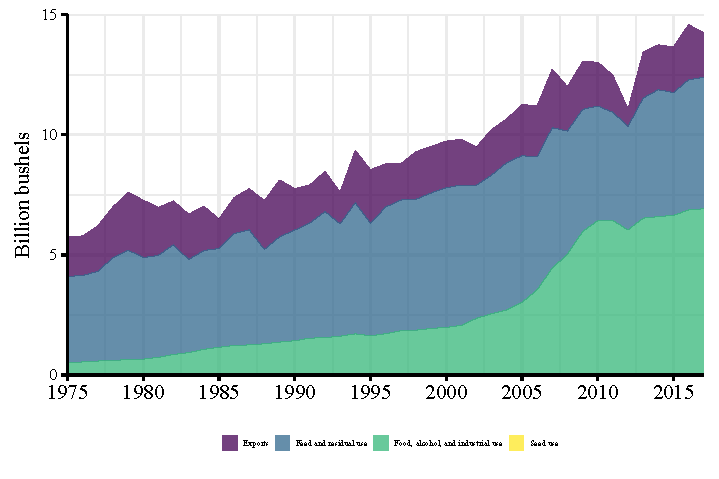
\includegraphics[width=\maxwidth]{figure/figure_use-1} 

\end{knitrout}
\scriptsize
Data source: \href{https://www.ers.usda.gov/data-products/feed-grains-database/feed-grains-yearbook-tables/}{ERS: Feed grains}.
\end{frame}

%%%%%%%%%%%%%%%%%%%%%%%%%%%%%%%%%%%%%%%%%%%%%%%%%%%%%%%%%%%%%%%%%%%%%%%%%%%%%%%%%%

\begin{frame}{Domestic use of corn - share}
\begin{knitrout}
\definecolor{shadecolor}{rgb}{0.969, 0.969, 0.969}\color{fgcolor}
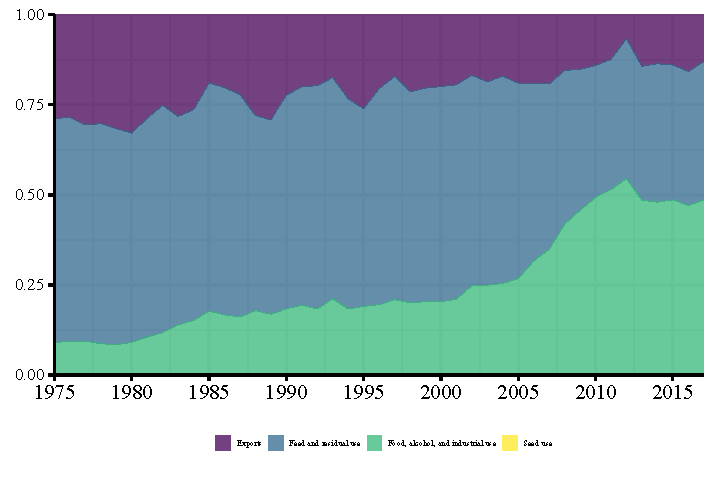
\includegraphics[width=\maxwidth]{figure/figure_share-1} 

\end{knitrout}
\scriptsize
Data source: \href{https://www.ers.usda.gov/data-products/feed-grains-database/feed-grains-yearbook-tables/}{ERS: Feed grains}.
\end{frame}


%%%%%%%%%%%%%%%%%%%%%%%%%%%%%%%%%%%%%%%%%%%%%%%%%%%%%%%%%%%%%%%%%%%%%%%%%%%%%%%%%%

\begin{frame}[allowframebreaks]{Stocks}
\begin{enumerate}[label=\textbullet]
  \item USDA September projections for the 2017-18 crop year are as follow
      \begin{enumerate}[label=-]
         \item Total supply of 16.585 billion bushels.
         \item Total use of 14.250 billion bushels.
         \item The difference between the supply and use gives a residual of 2.335 billion bushels.
         \item This represents the projected stock at the end of the 2017-18 crop year.
      \end{enumerate}  
  \item This means of a stock-to-use ratio of 100*2.335/14.250 = $16.39$. This is huge.
      \begin{enumerate}[label=-]
         \item 2012-13: ratio=7.4;
         \item 2013-14: ratio=9.1.
         \item 2014-15: ratio=15.23.
         \item 2015-16: ratio=11.35.
         \item 2016-17: ratio=16.47.
      \end{enumerate}
  \item One implication is that another good crop next summer will lead to low prices for corn in 2018.
\end{enumerate}
\end{frame}

%%%%%%%%%%%%%%%%%%%%%%%%%%%%%%%%%%%%%%%%%%%%%%%%%%%%%%%%%%%%%%%%%%%%%%%%%%%%%%%%%

\section{A small economic model}

\begin{frame}{Fundamental analysis: a small model of the US corn market}
\begin{enumerate}[label=\textbullet]
  \item We will use a small economic model.
  \item The role of the model is to summarize, within a mathematical structure, all the information that we have about the corn market.
  \item The model helps understand all the assumptions that enter into making a prediction/projection.
  \item We will look at what are the shapes of the supply and demand curves.
\end{enumerate}
\end{frame}

%%%%%%%%%%%%%%%%%%%%%%%%%%%%%%%%%%%%%%%%%%%%%%%%%%%%%%%%%%%%%%%%%%%%%%%%%%%%%%%%%

\begin{frame}{Fundamental analysis: a small model of the US corn market}
\begin{enumerate}[label=\textbullet]
  \item We will view the basic of fundamental analysis by modeling supply and demand curves for the corn market.
  \item \textcolor[rgb]{1.00,0.00,0.00}{We will pretend that we are May 2017 and that our objective is to \emph{forecast a range of prices} for the corn crop in the Fall of 2017.}
  \item We will then validate the price forecasted with the model with today's price.
\end{enumerate}
\end{frame}

%%%%%%%%%%%%%%%%%%%%%%%%%%%%%%%%%%%%%%%%%%%%%%%%%%%%%%%%%%%%%%%%%%%%%%%%%%%%%%%%%%

\begin{frame}{Fundamental analysis: application to the corn market}
\begin{enumerate}[label=\textbullet]
  \item Fundamental analysis for the corn market is fairly simple.
  \item Similar analyses for other grains tend to be more complicated because of trade. Modeling those markets would require the rest-of-the-world (countries other than the United States) supply and demand equations.
  \item Livestock requires a more complicated model because of the dynamic of production (e.g. cattle and hog cycles) and the importance of input costs.
\end{enumerate}
\end{frame}

%%%%%%%%%%%%%%%%%%%%%%%%%%%%%%%%%%%%%%%%%%%%%%%%%%%%%%%%%%%%%%%%%%%%%%%%%%%%%%%%%%

\begin{frame}{Supply of corn}
\begin{enumerate}[label=\textbullet]
  \item The supply of corn is almost perfectly inelastic after planting.
  \item The supply is not perfectly inelastic because of storage carrying over from one year to the other and because of trade.
  \item As we are interested in a forecast for a period less than one year, so assuming a perfectly inelastic supply of corn between May and November is reasonable.
\end{enumerate}
\end{frame}

%%%%%%%%%%%%%%%%%%%%%%%%%%%%%%%%%%%%%%%%%%%%%%%%%%%%%%%%%%%%%%%%%%%%%%%%%%%%%%%%%%

\begin{frame}{Demand for corn}
\begin{enumerate}[label=\textbullet]
  \item What value to use for the elasticity of demand for corn?
  \item It is difficult to find the correct estimate of the elasticity of demand for a product.
  \item Typically, an elasticity of demand for corn for that time frame of $-0.3$ is reasonable and been used by other.
  \item To verify the sensitivity of the results, let's also use alternative values for the elasticity of demand of $-0.2$ and $-0.4$.
\end{enumerate}
\end{frame}

%%%%%%%%%%%%%%%%%%%%%%%%%%%%%%%%%%%%%%%%%%%%%%%%%%%%%%%%%%%%%%%%%%%%%%%%%%%%%%%%%%

\begin{frame}{Market equilibrium}
\begin{enumerate}[label=\textbullet]
  \item Now, we have a good idea of the slopes (elasticities) of supply and demand curves.
  \item To predict the corn market in the Fall, we derive an expression for the demand curve.
  \item One simple method is to calculate parameters of a linear demand function using observed prices and quantities.
  \item Thus, we need information about prices and quantities.
\end{enumerate}
\end{frame}


%%%%%%%%%%%%%%%%%%%%%%%%%%%%%%%%%%%%%%%%%%%%%%%%%%%%%%%%%%%%%%%%%%%%%%%%%%%%%%%%%%

\begin{frame}{The price}
\begin{enumerate}[label=\textbullet]
  \item The WASDE report gives us a projection of the quantity supplied and the price.
  \item The WASDE report gives a projection of the \emph{farm} price of corn for the crop/marketing year. This is not what we want.
  \item What we want is the 2016 December futures corn price when the prediction takes place.
  \item The reason to use the December corn futures is that it represents what the market thinks the price of corn will be in December. It is also the futures contract that expires soon after harvest.
  \item Cash prices are based on futures prices.
  \end{enumerate}
\end{frame}
%%%%%%%%%%%%%%%%%%%%%%%%%%%%%%%%%%%%%%%%%%%%%%%%%%%%%%%%%%%%%%%%%%%%%%%%%%%%%%%%%%

\begin{frame}{What price and data to use to calibrate the demand?}
\begin{enumerate}[label=\textbullet]
  \item Remember that we are trying to do a forecast pretending that we are in May 2017.
  \item We can use only information that was available in May 2017.
  \item In May 2017, the WASDE reported projected a total supply of corn of 16.410 billion bushels of corn for 2017.
  \item In the week of the release of the May 2017 WASDE report, the price of corn average \textcent 388.13 per bushel.
\end{enumerate}
\end{frame}

%%%%%%%%%%%%%%%%%%%%%%%%%%%%%%%%%%%%%%%%%%%%%%%%%%%%%%%%%%%%%%%%%%%%%%%%%%%%%%%%%%
\subsection{Calculating the demand curve}

\begin{frame}{Calculating the demand curve}
\begin{enumerate}[label=\textbullet]
  \item We will calculate the parameters of a linear demand based on the data we observe and values for the elasticity of demand.
  \item The functional form for the demand curve is:\[ Q = a - b P, \] where $a>0$ and $b>0$ are parameters of the demand function.
  \item Recall that we can calculate the parameter $b$ based on the value for the elasticity of demand: \[b = -\eta \frac{Q^d}{P}.\]
  \vspace{-\baselineskip}
  \item After calculating $b$, we can then calculate a value for $a$ as $a = Q - b P$.
\end{enumerate}
\end{frame}

%%%%%%%%%%%%%%%%%%%%%%%%%%%%%%%%%%%%%%%%%%%%%%%%%%%%%%%%%%%%%%%%%%%%%%%%%%%%%%%%%%

\begin{frame}{Calculating the demand curve}
\begin{enumerate}[label=\textbullet]
  \item The calibration of the demand uses a total quantity of corn of 16.410 billion bushels and a futures price of December corn of \textcent 388.13 per bushel.
  \item Let's do the calculations here assuming that the elasticity of demand is $\eta=-0.4$.
  \item The value of the parameter $b$ is \[b = -\eta \frac{Q}{P} = 0.4 \frac{16.410}{388.13} = 0.0169.\]
  \vspace{-\baselineskip}
  \item The value of the parameter $a$ is \[a = Q + b P = 16.410 + 0.0169*388.13 = 22.974.\]
\end{enumerate}
\end{frame}

%%%%%%%%%%%%%%%%%%%%%%%%%%%%%%%%%%%%%%%%%%%%%%%%%%%%%%%%%%%%%%%%%%%%%%%%%%%%%%%%%%

\begin{frame}{Calculating the demand curve}
\begin{table}
\caption{Demand parameters}
\scriptsize
\begin{tabular}{l c c c}
  \toprule
   & $\eta=-0.2$ & $\eta = -0.3$ & $\eta=-0.4$ \\
   \midrule
   $a$ & 19.692 & 21.333 & 22.974 \\
   $b$ & 0.0085 & 0.0127 & 0.0169 \\
  \bottomrule
\end{tabular}
\end{table}
\end{frame}

%%%%%%%%%%%%%%%%%%%%%%%%%%%%%%%%%%%%%%%%%%%%%%%%%%%%%%%%%%%%%%%%%%%%%%%%%%%%%%%%%%

\begin{frame}{Demand curves for corn}
\begin{knitrout}
\definecolor{shadecolor}{rgb}{0.969, 0.969, 0.969}\color{fgcolor}
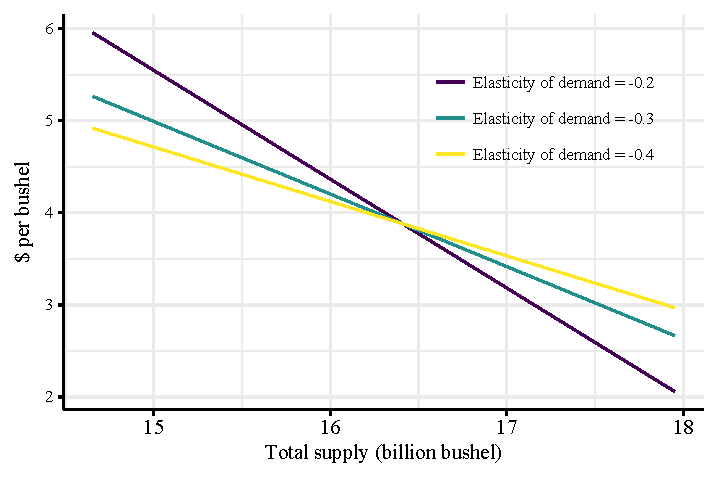
\includegraphics[width=\maxwidth]{figure/figure_demand-1} 

\end{knitrout}
\end{frame}

%%%%%%%%%%%%%%%%%%%%%%%%%%%%%%%%%%%%%%%%%%%%%%%%%%%%%%%%%%%%%%%%%%%%%%%%%%%%%%%%%%

\begin{frame}[allowframebreaks]{Demand curve in function of yield}
\begin{enumerate}[label=\textbullet]
  \item The previous figure shows demand lines in function of the total quantity of corn.
  \item For some people, it is however easier to think in terms of yield.
  \item Yield is also the most significant source of uncertainty. Thus, a prediction conditional on corn yield is relevant.
  \item The total quantity supplied ($Q$) is equal to the harvest ($H$), plus the corn in storage at the beginning of the crop year ($S$): \[ Q = H + S. \]
  \vspace{-\baselineskip}
  \item Imports are negligible and ignored.
  \item The May 2017 WASDE reported beginning stock of 2.295 billion bushels. So, let's assume this number as the beginning stock ($S=2.295$).
  \item The harvest ($H$) is simply the product of the acres harvested($A$) and the yield ($y$): \[ H = A*y.\]
  \vspace{-\baselineskip}
  \item Thus, we can write that: \[ A*y = Q - S.\]
  \vspace{-\baselineskip}
  \item Thus from the previous expression, we can recover the implied yield from a given total supply as \[ y = \frac{Q-S}{A}.\]
  \vspace{-\baselineskip}
  \item In May 2017, WASDE predicted harvested acreage for corn of 82.4 million acres for 2017. So, let's use $A=82.4$.
  \item Now, we can calculate the implied yield from a total quantity of corn supplied.
  \item For example, if the total quantity supplied is 16 billion bushels, we can calculate that the implied yield in bushels per acre is \[ y = 1000*\frac{16-2.295}{82.4} = 166.3.\]
\end{enumerate}
\end{frame}

%%%%%%%%%%%%%%%%%%%%%%%%%%%%%%%%%%%%%%%%%%%%%%%%%%%%%%%%%%%%%%%%%%%%%%%%%%%%%%%%%%

\begin{frame}{Demand curves in function of yield}
\begin{knitrout}
\definecolor{shadecolor}{rgb}{0.969, 0.969, 0.969}\color{fgcolor}
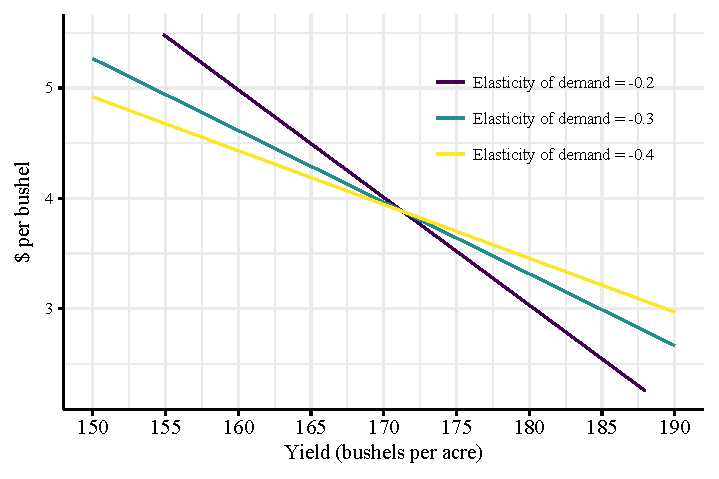
\includegraphics[width=\maxwidth]{figure/figure_demand2-1} 

\end{knitrout}
\end{frame}

%%%%%%%%%%%%%%%%%%%%%%%%%%%%%%%%%%%%%%%%%%%%%%%%%%%%%%%%%%%%%%%%%%%%%%%%%%%%%%%%%%


\subsection{Predicting the price of corn}

\begin{frame}{Prediction: what corn yield to use?}
\begin{enumerate}[label=\textbullet]
  \item Corn yield is the main source of uncertainty in performing this prediction.
  \item In May 2017, WASDE projected a yield of 170.7 bushels per acre for the 2017 corn crop.
  \item Typically, projections use trend yields.
  \item Let's look at historical data on corn yields.
\end{enumerate}
\end{frame}

%%%%%%%%%%%%%%%%%%%%%%%%%%%%%%%%%%%%%%%%%%%%%%%%%%%%%%%%%%%%%%%%%%%%%%%%%%%%%%%%%%

\begin{frame}{Historical corn yields}
\begin{knitrout}
\definecolor{shadecolor}{rgb}{0.969, 0.969, 0.969}\color{fgcolor}
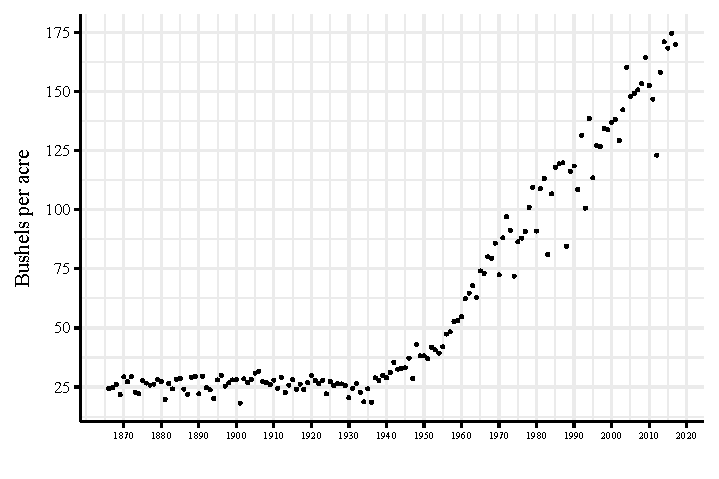
\includegraphics[width=\maxwidth]{figure/figure_corn_yield-1} 

\end{knitrout}
\scriptsize
Data source: \url{http://www.nass.usda.gov/Statistics_by_Subject/index.php}.
\end{frame}

%%%%%%%%%%%%%%%%%%%%%%%%%%%%%%%%%%%%%%%%%%%%%%%%%%%%%%%%%%%%%%%%%%%%%%%%%%%%%%%%%%

\begin{frame}{Historical corn yields - with trend}
\begin{knitrout}
\definecolor{shadecolor}{rgb}{0.969, 0.969, 0.969}\color{fgcolor}
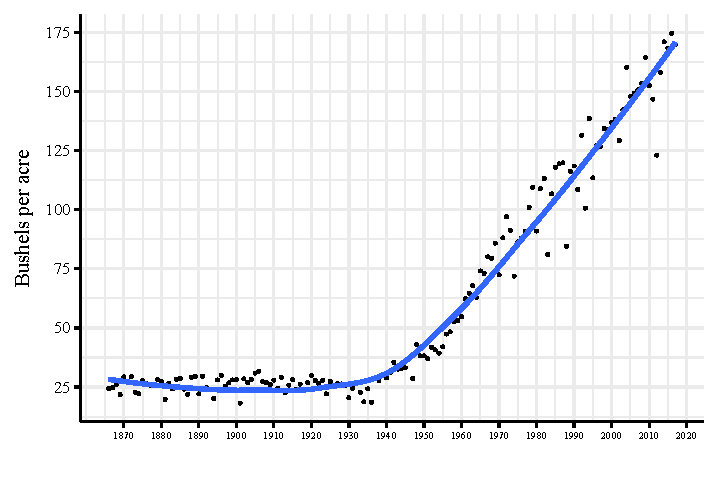
\includegraphics[width=\maxwidth]{figure/figure_corn_yield2-1} 

\end{knitrout}
\scriptsize
Data source: \url{http://www.nass.usda.gov/Statistics_by_Subject/index.php}.
\end{frame}

%%%%%%%%%%%%%%%%%%%%%%%%%%%%%%%%%%%%%%%%%%%%%%%%%%%%%%%%%%%%%%%%%%%%%%%%%%%%%%%%%%

\begin{frame}{Recent percentage deviations in corn yields from trend}
\begin{knitrout}
\definecolor{shadecolor}{rgb}{0.969, 0.969, 0.969}\color{fgcolor}
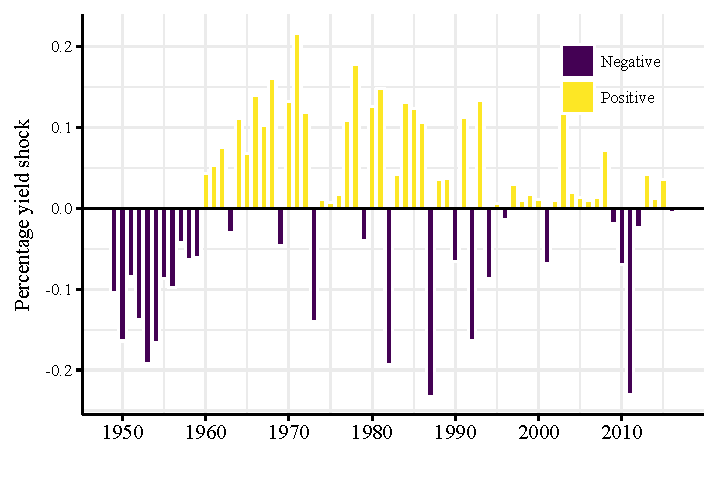
\includegraphics[width=\maxwidth]{figure/figure_percent-1} 

\end{knitrout}
\end{frame}

%%%%%%%%%%%%%%%%%%%%%%%%%%%%%%%%%%%%%%%%%%%%%%%%%%%%%%%%%%%%%%%%%%%%%%%%%%%%%%%%%%

\begin{frame}{Prediction: what corn yield to use?}
\begin{enumerate}[label=\textbullet]
  \item From the previous slide, a trend yield of 170 bushels per acre is reasonable.
  \item For a sensitivity analysis, let's use alternative corn yields of 150 and 175 bushels per acre.
\end{enumerate}
\begin{table}
\caption{Corn yield expectation}
\begin{tabular}{c c c}
  \toprule
   Min & Median & Max \\
   150 & 170 & 175\\
  \bottomrule
\end{tabular}
\end{table}
\end{frame}

%%%%%%%%%%%%%%%%%%%%%%%%%%%%%%%%%%%%%%%%%%%%%%%%%%%%%%%%%%%%%%%%%%%%%%%%%%%%%%%%%%

\begin{frame}{Prediction using median expected yield}
\begin{enumerate}[label=\textbullet]
  \item Let me do an example of the calculations assuming a yield of 170 bushels per acre.
  \item Given the assumption on the yield and assuming that harvested acreage equals the WASDE projection, the harvest would be 170 bushel per acre * 82.4 million acres = 14.008 billion bushels.
  \item We can add to the harvest USDA May 2017 stock prediction of 2.295 billion bushels to find a total supply of corn of 14.008 + 2.295 = 16.303 billion bushels.
\end{enumerate}
\end{frame}

%%%%%%%%%%%%%%%%%%%%%%%%%%%%%%%%%%%%%%%%%%%%%%%%%%%%%%%%%%%%%%%%%%%%%%%%%%%%%%%%%%

\begin{frame}{Prediction using median expected yield}
\begin{enumerate}[label=\textbullet]
  \item I will show the calculations using the demand curve with an elasticity of $-0.4$.
  \item To predict the price, we must use the inverse demand function:  \[ P = \frac{(a - Q)}{b}. \]
  \vspace{-\baselineskip}
  \item Thus, from our assumptions on yield, acreage and elasticity, we can predict that the price of corn will be: \[ \frac{(22.974 - 16.303)}{0.0169} = \$3.94/bu.\]
  \vspace{-\baselineskip}
  \item We can repeat these calculations with other values for the elasticity of demand and for other values for the expected yield.
\end{enumerate}
\end{frame}

%%%%%%%%%%%%%%%%%%%%%%%%%%%%%%%%%%%%%%%%%%%%%%%%%%%%%%%%%%%%%%%%%%%%%%%%%%%%%%%%%%

\begin{frame}{Predictions for the price of corn}\label{slide.tab}
\begin{table}
\caption{Prices prediction with expected yield}
\begin{tabular}{c c c c}
  \toprule
  Yield (bu/acre) & $\eta=-0.2$ & $\eta=-0.3$ & $\eta=-0.4$ \\
   \midrule
   150  & $\$5.96 /bu$ & $\$5.26 /bu$ & $\$4.91 /bu$ \\
   170 & $\$4.01 /bu$ & \textbf{$\$3.97 /bu$} & $\$3.94 /bu$ \\
   175  & $\$3.52 /bu$ & $\$3.64 /bu$ & $\$3.70 /bu$ \\
  \bottomrule
\end{tabular}
\end{table}
\end{frame}

%%%%%%%%%%%%%%%%%%%%%%%%%%%%%%%%%%%%%%%%%%%%%%%%%%%%%%%%%%%%%%%%%%%%%%%%%%%%%%%%%%

\begin{frame}{What does it say?}
\begin{enumerate}[label=\textbullet]
  \item The prediction assuming 170 bushels per acre and an elasticity of -0.3 says that the price of corn in Fall 2017 would be about $\$3.97 /bu$.
  \item Lower yield at 150 bushels per acre causes the price to increase by more than a \$1.00 per bushel.
  \item Higher yield at 175 bushels per acre causes the price to decline by about \$0.50 per bushel.
\end{enumerate}
\end{frame}

%%%%%%%%%%%%%%%%%%%%%%%%%%%%%%%%%%%%%%%%%%%%%%%%%%%%%%%%%%%%%%%%%%%%%%%%%%%%%%%%%%

\begin{frame}{Demand curves in function of yield}
\begin{knitrout}
\definecolor{shadecolor}{rgb}{0.969, 0.969, 0.969}\color{fgcolor}
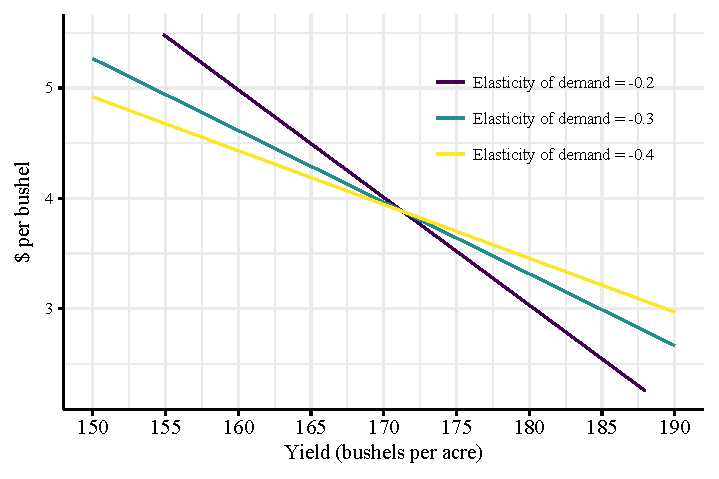
\includegraphics[width=\maxwidth]{figure/figure_demand_plot-1} 

\end{knitrout}
\end{frame}


%%%%%%%%%%%%%%%%%%%%%%%%%%%%%%%%%%%%%%%%%%%%%%%%%%%%%%%%%%%%%%%%%%%%%%%%%%%%%%%%%%

\begin{frame}{Elasticity of supply}
\begin{enumerate}[label=\textbullet]
  \item The supply of corn is assumed perfectly inelastic.
        \begin{enumerate}[label=-]
         \item Could repeat the prediction using an elasticity of supply of $0.1$.
        \end{enumerate}
  \item The assumption regarding yield is the one that influences the prediction the most.
        \begin{enumerate}[label=-]
         \item The prediction assumes corn yield that is typical of what has been observed in recent years.
        \end{enumerate}
\end{enumerate}
\end{frame}

%%%%%%%%%%%%%%%%%%%%%%%%%%%%%%%%%%%%%%%%%%%%%%%%%%%%%%%%%%%%%%%%%%%%%%%%%%%%%%%%%%

\subsection{In retrospect}

\begin{frame}{What does the model mean?}
\begin{enumerate}[label=\textbullet]
  \item The simple model summarizes (quantifies) all information about the market into one equation for the demand.
  \item The information missing is regarding production, i.e. yield.
  \item Thus, given the model, the only data to input is yield, which is the variable with the most uncertainty.
\end{enumerate}
\end{frame}

%%%%%%%%%%%%%%%%%%%%%%%%%%%%%%%%%%%%%%%%%%%%%%%%%%%%%%%%%%%%%%%%%%%%%%%%%%%%%%%%%%

\begin{frame}{How well does the simple prediction perform?}\label{slide.retro}
\begin{enumerate}[label=\textbullet]
  \item Retrospectively, we can look at how well the forecast worked.
  \item The next two slides show the demand curves and a point for the futures price in September 2017 and the yield reported in the September 2017 WASDE reports.
  \item The model is off by about \$0.40/bu. That is quite a lot. In previous years, this simple model had worked much better.
  \item An explanation is that the market did not believe the earlier yield estimates from the USDA, which happened to be quite accurate. 
\end{enumerate}
\end{frame}

%%%%%%%%%%%%%%%%%%%%%%%%%%%%%%%%%%%%%%%%%%%%%%%%%%%%%%%%%%%%%%%%%%%%%%%%%%%%%%%%%%

\begin{frame}{Demand curves in function of yield}
\begin{knitrout}
\definecolor{shadecolor}{rgb}{0.969, 0.969, 0.969}\color{fgcolor}
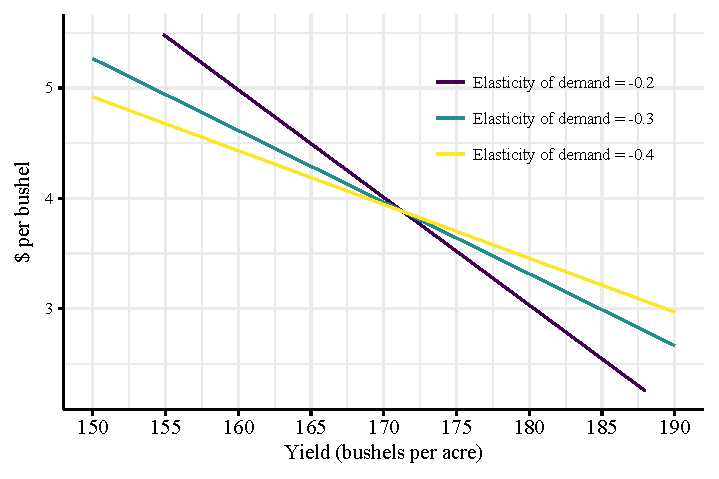
\includegraphics[width=\maxwidth]{figure/figure_demand_plot2-1} 

\end{knitrout}
\end{frame}

%%%%%%%%%%%%%%%%%%%%%%%%%%%%%%%%%%%%%%%%%%%%%%%%%%%%%%%%%%%%%%%%%%%%%%%%%%%%%%%%%%

\begin{frame}{Demand curves in function of yield with 2017 data}
\begin{knitrout}
\definecolor{shadecolor}{rgb}{0.969, 0.969, 0.969}\color{fgcolor}
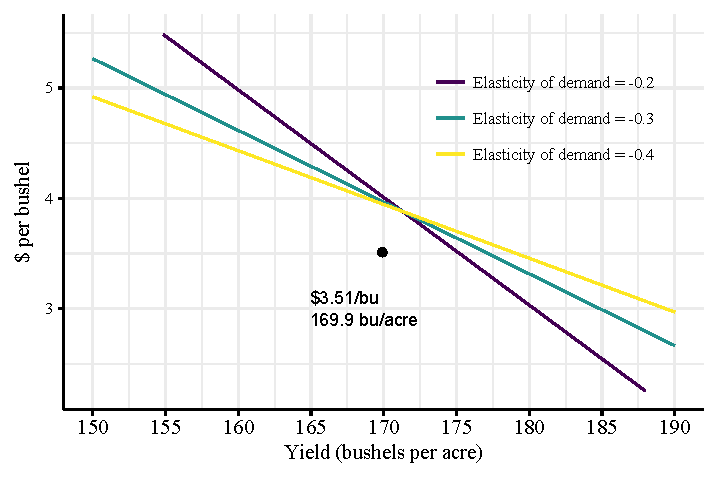
\includegraphics[width=\maxwidth]{figure/figure_retro-1} 

\end{knitrout}
\end{frame}

%%%%%%%%%%%%%%%%%%%%%%%%%%%%%%%%%%%%%%%%%%%%%%%%%%%%%%%%%%%%%%%%%%%%%%%%%%%%%%%%%%

\begin{frame}{Price of the December 2017 futures contract}
\begin{knitrout}
\definecolor{shadecolor}{rgb}{0.969, 0.969, 0.969}\color{fgcolor}
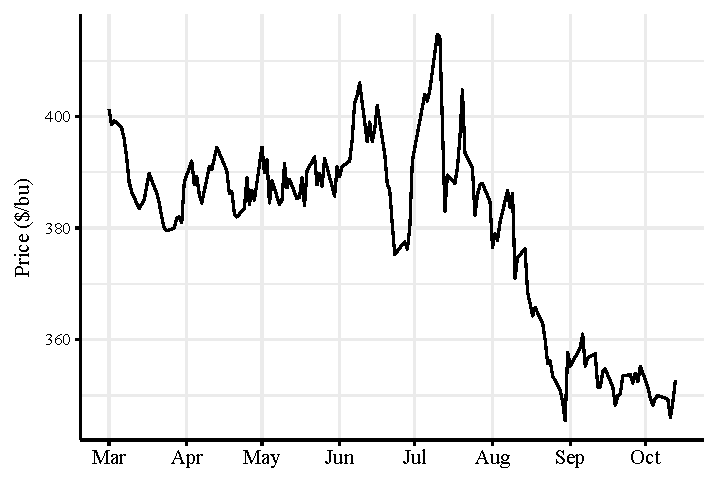
\includegraphics[width=\maxwidth]{figure/figure_corn-1} 

\end{knitrout}
\end{frame}

%%%%%%%%%%%%%%%%%%%%%%%%%%%%%%%%%%%%%%%%%%%%%%%%%%%%%%%%%%%%%%%%%%%%%%%%%%%%%%%%%%

\begin{frame}[allowframebreaks]{Can we say something about 2018?}
\begin{enumerate}[label=\textbullet]
  \item Suppose that the stock of corn on October 2018 equals the stock projected in the latest WASDE report: 2.335 billion bushels.
  \item Given the low prices for corn and soybeans, it would not be surprising that the area harvested of corn next year to be low. Suppose that next summer that the total area harvested of corn equals 83 million acres.
  \item Suppose that next year corn yields are right along the trend at 170 bushels per acre.
  \item In total, it means for next year a total supply of corn of 83*170/1000 + 2.335 = 16.445 billion bushels.
  \item With the demand derived using an elasticity of -0.3, the projected price for corn in Fall 2017 is \$3.83 per bushel.
  \item If the yield is 175 bushels per acre, then the projected price goes down to \$3.60 per bushel.
  \item If the area harvested is 83 million acres and the yield is 170 bushels per acre, then the project price is \$3.53 per bushel.
  \item These projections are likely too high because they are based on a calibration price of \$3.88/bu that was observed last May. A price of closed to what has been observed lately, about \$3.50/bu, would work better.
  \item It is quite early to project corn price for Fall 2018. We can say however that if the crop next year is decent that the price of corn will be less than \$4 per bushel. With another bumper crop, it could even be closed to \$3 per bushel.
  \item What is the futures price for corn for December 2018?
  \item What could change between now and December 2018? NAFTA...
\end{enumerate}
\end{frame}


%%%%%%%%%%%%%%%%%%%%%%%%%%%%%%%%%%%%%%%%%%%%%%%%%%%%%%%%%%%%%%%%%%%%%%%%%%%%%%%%%%

\begin{frame}{Other commodities}
\begin{enumerate}[label=\textbullet]
  \item For other agricultural commodities this simple framework might not work as well:
        \begin{enumerate}[label=-]
            \item Change in supply and demand conditions because of trade;
            \item Production dynamic.
        \end{enumerate}
  \item The prices of some commodities are linked through fairly constant ratios:
        \begin{enumerate}[label=-]
            \item This reflects that these commodities are substitutes in supply and/or demand.
        \end{enumerate}
\end{enumerate}
\end{frame}


%%%%%%%%%%%%%%%%%%%%%%%%%%%%%%%%%%%%%%%%%%%%%%%%%%%%%%%%%%%%%%%%%%%%%%%%%%%%%%%%%%

\begin{frame}{Soybean to corn price ratio}
\begin{knitrout}
\definecolor{shadecolor}{rgb}{0.969, 0.969, 0.969}\color{fgcolor}
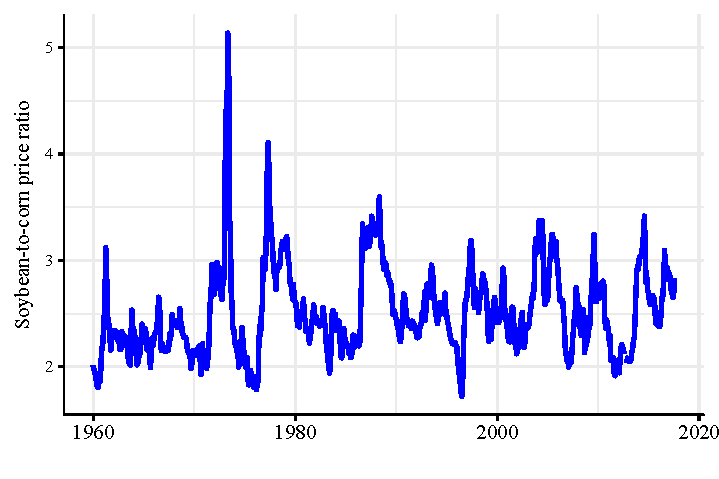
\includegraphics[width=\maxwidth]{figure/figure_ratio-1} 

\end{knitrout}
\scriptsize
Source: Price data were downloaded from \url{http://farmdoc.illinois.edu/manage/uspricehistory/us_price_history.html}.
\end{frame}

%%%%%%%%%%%%%%%%%%%%%%%%%%%%%%%%%%%%%%%%%%%%%%%%%%%%%%%%%%%%%%%%%%%%%%%%%%%%%%%%%%

\begin{frame}{Prediction for the price of soybeans}
\begin{enumerate}[label=\textbullet]
  \item Since 1960, the soybean-corn price ratio has been on average 2.51.
  \item Since 2000, the soybean-corn price ratio has also been on average 2.56.
  \item Based on that ratio, it is possible to make a simple prediction of the price of soybeans.
  \item For example, at the forecast of \$3.97/bu, the ratio implies a \$10.16/bu for soybean.
  \item That forecast will however be less precise as there is also uncertainty regarding the value of the ratio.
  \item The soybean-corn price ratio is a rule of thumb that has been losing favor.
\end{enumerate}
\end{frame}

%%%%%%%%%%%%%%%%%%%%%%%%%%%%%%%%%%%%%%%%%%%%%%%%%%%%%%%%%%%%%%%%%%%%%%%%%%%%%%%%%%

\begin{frame}{FYI - soybeans historical yields}
\begin{knitrout}
\definecolor{shadecolor}{rgb}{0.969, 0.969, 0.969}\color{fgcolor}
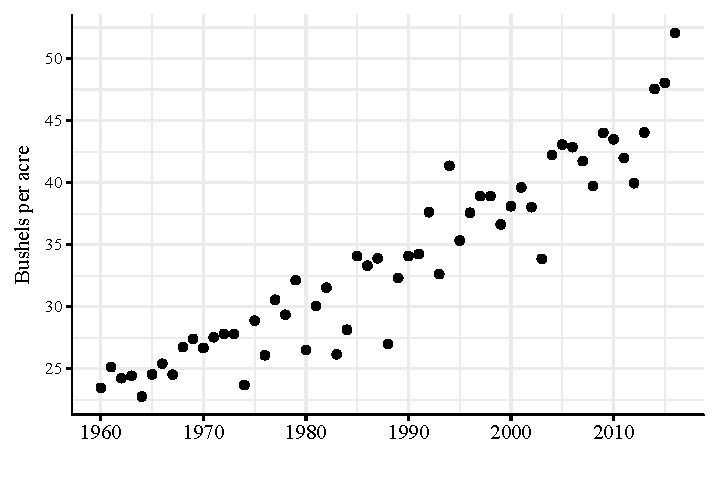
\includegraphics[width=\maxwidth]{figure/figure_soybean_yield-1} 

\end{knitrout}
\scriptsize
Data source: \url{http://www.nass.usda.gov/Statistics_by_Subject/index.php}.
\end{frame}

%%%%%%%%%%%%%%%%%%%%%%%%%%%%%%%%%%%%%%%%%%%%%%%%%%%%%%%%%%%%%%%%%%%%%%%%%%%%%%%%%%

\begin{frame}{FYI - soybeans historical yields}
\begin{knitrout}
\definecolor{shadecolor}{rgb}{0.969, 0.969, 0.969}\color{fgcolor}
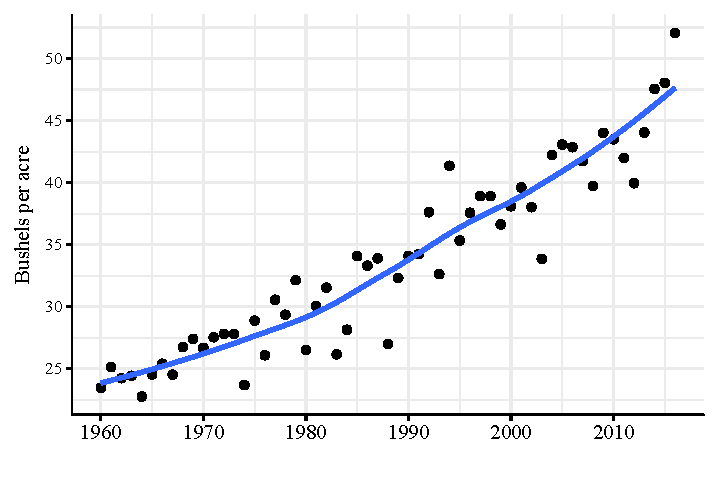
\includegraphics[width=\maxwidth]{figure/figure_soybean_yield2-1} 

\end{knitrout}
\scriptsize
Data source: \url{http://www.nass.usda.gov/Statistics_by_Subject/index.php}.
\end{frame}

%%%%%%%%%%%%%%%%%%%%%%%%%%%%%%%%%%%%%%%%%%%%%%%%%%%%%%%%%%%%%%%%%%%%%%%%%%%%%%%%%%

\section{Quality of prediction}

\begin{frame}[allowframebreaks]{Can we trust predictions/projections?}
\begin{enumerate}[label=\textbullet]
  \item \textbf{Prediction:} a statement about the way things will happen in the future that might be based on experience and knowledge.
  \item \textbf{Projection:} an estimate of a future situation based on a study of a present situation.
  \item What we want is a projection that offers a description of what will happen in the future conditional on the conditions currently observed.
  \item Projections are an effort to foresee what is going to happen in the future.
  \framebreak
  \item A prediction or a projection should always come with a time stamp and an expiration date.
        \begin{enumerate}[label=-]
         \item A prediction uses information available at a specific date. Soon after, that information may no longer be true.
         \item If there is no expiration date to a prediction, a prediction like this is always correct: ``Iowa State Cyclone will one day win the College Football Playoff National Championship.''
         \item A statement such as ``Iowa State Cyclone will win the College Football Playoff National Championship by 2022'' is much more meaningful.
        \end{enumerate}
  \item A projection is good if it derives from reasonable assumptions and from the correct model.
  \pagebreak
  \item If only one assumption does not hold, then the projection will not materialize.
        \begin{enumerate}[label=-]
         \item The case of the 2012 corn crop with the drought is a good example.
         \item There are always a lot of assumptions in one projection. Given all those assumptions, how can someone put any trust into a projection?
        \end{enumerate}
  \item Markets are difficult to project as there are a lot of variables to take into account.
  \framebreak
  \item Those that make predictions/projections are not held accountable for bad forecast.
        \begin{enumerate}[label=-]
         \item Someone who made a correct prediction will brag about it while someone who made a wrong prediction will keep quiet.
         \item There is little to no punishment to those who make wrong predictions while a correct prediction may receive a lot of press coverage.
         \end{enumerate}
  \item Media tend to seek people who make bold prediction/projection because they are more entertaining.
    \begin{enumerate}[label=-]
        \item \href{http://www.freakonomics.com/2011/09/14/new-freakonomics-radio-podcast-the-folly-of-prediction/}{Listen} or \href{http://www.freakonomics.com/2011/06/30/the-folly-of-prediction-full-transcript/}{read} the Freakonomics podcast titled ``The Folly of Prediction'' for some discussion about this.
      \end{enumerate}
\end{enumerate}
\end{frame}

%%%%%%%%%%%%%%%%%%%%%%%%%%%%%%%%%%%%%%%%%%%%%%%%%%%%%%%%%%%%%%%%%%%%%%%%%%%%%%%%%%

\begin{frame}{What is the value of a prediction?}
\begin{enumerate}[label=\textbullet]
  \item For a speculator, a projection about future prices can be very valuable.
        \begin{enumerate}[label=-]
            \item Speculation is all about taking risk to gain profit from variations, or non-variations, in prices.
        \end{enumerate}
  \item For a hedger, the issue is more regarding the probability that a price rises or declines.
        \begin{enumerate}[label=-]
            \item The objective should then be about knowing the risk that the price goes beyond a certain threshold rather than knowing exactly what the price is going to be.
            \item Although a projection can be valuable, it is understanding the events that affect a price that matter the most and understanding how likely those events are to happen.
        \end{enumerate}
\end{enumerate}
\end{frame}


%%%%%%%%%%%%%%%%%%%%%%%%%%%%%%%%%%%%%%%%%%%%%%%%%%%%%%%%%%%%%%%%%%%%%%%%%%%%%%%%%%

\begin{frame}{What to make of predictions/projections?}
\begin{enumerate}[label=\textbullet]
    \item Given all the uncertainty, can you fully trust a prediction/projection when making decisions?
  \item You are the judge!
\end{enumerate}
\end{frame}


%%%%%%%%%%%%%%%%%%%%%%%%%%%%%%%%%%%%%%%%%%%%%%%%%%%%%%%%%%%%%%%%%%%%%%%%%%%%%%%%%%%%
\section[References]{References}
\renewcommand\refname{References}
\def\newblock{References}
\begin{frame}{References}
\bibliography{D:/Dropbox/Papers/References}
%\bibliography{D:/Papers/References}
\end{frame}


%%%%%%%%%%%%%%%%%%%%%%%%%%%%%%%%%%%%%%%%%%%%%%%%%%%%%%%%%%%%%%%%%%%%%%%%%%%%%%%%%%%%%

\end{document}
